\chapter{Controlling Weakly-coupled Carbon Spins}
[Note intro needs to be rewritten once chapter is done]\\
Now that we have identified several promising carbon spins we will go into controlling them.
This chapter attempts to explain first how we can control a carbon by explaining how the two different rotation axes from the last chapter can be used to implement a conditional +-X gate. A gate similar to a CNOT gate.
Now that we understand how to implement a cnot gate we will use this to perform an experiment that we call a carbon ramsey on an unitialized state.
AFterwards we will use this to show that we can initialize and readout by showing an initialized carbon ramsey. (1buit tomo (ramsey with more T +Z-RO?).
From this we will also determine $T_{2 \mathrm{C}}^*$.

The next section will consider two qubit control.
It will start by explaining how we can perform a parity measurement. This measurement allows us to perform a two qubit tomography and create entanglement by projection.
We will then show

\section{Controlling a single-carbon}
This section will explain how a weakly-coupled spin can be controlled using the conditional rotation of the carbon spin that occurs when on resonance (\cref{eq:res_dip_loc}).
It will start by explaining how to do basic gate operations in the ideal case of being perfectly on resonant and not interacting with any nuclear spins.
After that we will explain how a carbon-spin in a mixed state can be initialized

\subsection{Basic gates}
As was explained in \cref{sec:controllingacarbonthroughdynamicaldecoupling} nuclear spins perform a rotation along two anti-parallel axes when subjected to a dynamical decoupling sequence on a resonant condition given by \cref{eq:res_dip_loc}. The angle of this rotation can be controlled by choosing the number of pulses of the decoupling sequence. By choosing the number of pulses such that all coherence is lost when performing a dynamical decoupling spectroscopy measurement on the resonance a rotation of $+\pi/2$ along the x-direction is performed when the electron is in the $\ket{0}$-state and a $-\pi/2$-rotation along the x-axis is performed when the electron is in the $\ket{0}$-state.

We call this conditional rotation the $\pm \mathrm{x}$-gate and it forms the basis of our control over weakly coupled spins. \Cref{fig:gate_circuit_pm-x} shows how we depict the $\pm \mathrm{x}$-gate in a circuit-diagram.
An unconditional gate can be implemented by placing the electron in an eigenstate before performing the $\pm\mathrm{x}$-operation.
A $\pm{\mathrm{y}}$-gate is implemented by letting the phase evolve before implementing a $\pm{\mathrm{x}}$-gate (\cref{fig:gate_circuit_carbon_phase}).

\begin{figure}[htbp]
    \begin{subfigure}[t]{0.49\textwidth}
    \centering
        \mbox{
        \Qcircuit @C=1em @R=.7em {
         \lstick{\ket{\Psi}_e} &\ctrl{1}  &\qw\\
          \lstick{\ket{\Psi}_\mathrm{C}} &\gate{\pm \mathrm{x} }  &\qw}}
        \caption{The conditional x-gate ($\pm\mathrm{x}$).}
        \label{fig:gate_circuit_pm-x}
    \end{subfigure}
    \begin{subfigure}[t]{0.49\textwidth}
        \centering
        \mbox{
        \Qcircuit @C=1em @R=.7em {
          &\ctrl{1}  &\qw &\dstick{=} &&\qw& \ctrl{1} &\qw \\
          &\gate{\pm \mathrm{y} }  &\qw &&& \gate{\mathrm{z}}  &\gate{\pm \mathrm{x} } &\qw}}
        \caption{The conditional y-gate ($\pm\mathrm{y}$).}
        \label{fig:gate_circuit_carbon_phase}
    \end{subfigure}
    \label{fig:basic_carbon_gates}
    \caption{\Cref{fig:gate_circuit_pm-x} The conditional x-gate ($\pm\mathrm{x}$). Performs an x-rotation on the carbon state ($\ket{\Psi }_\mathrm{C}$) when the electron is in the $\ket{0}_e$-state. It performs a $-\mathrm{x}$ rotation when the electron is in the $\ket{1}_e$-state. \Cref{fig:gate_circuit_carbon_phase} The conditional y-gate ($\pm\mathrm{y}$) is implemented by letting the phase evolve before performing a conditional x rotation ($\pm\mathrm{x}$) on the carbon.}
\end{figure}

\subsection{Initializing a carbon-spin}
We can use the $\pm\mathrm{x}$-gate to initialize a carbon-spin in the $ \ket{X}$-state.
For this we implement the gate-circuit as depicted in \cref{fig:gate_circuit_mbi_x-init}.
After the electron is brought in the $\ket{X}$ the state can be described by the tensor product of two density matrices:
\begin{equation}
    \rho_X \otimes \rho_m = \rho_X \otimes \rho_{X} +\rho_X \otimes \rho_{-X}
\end{equation}
Where the electron picks up a phase due to the $\pm{\mathrm{x}}$-gate depending on the nuclear spin-state:
\begin{equation}
     \rho_Y \otimes \rho_{X} +\rho_{-Y} \otimes \rho_{X}
    \label{eq:density_after_Ren}
\end{equation}

The effect of the $\pm{\mathrm{x}}$-gate can be made more easily understood by treating the carbon-spin as being either in the $\ket{X}$ or $\ket{-X}$-state.
\begin{align}
    \ket{X}\ket{X} \quad \vee  \quad\ket{X}\ket{-X}\\
    \frac{\ket{0}+\ket{1}}{\sqrt{2}}\ket{X} \quad \vee \quad \frac{\ket{0}+\ket{1}}{\sqrt{2}}\ket{-X} \\
    \frac{e^{-i\pi/4}\ket{0}+e^{i\pi/4}\ket{1}}{\sqrt{2}}\ket{X} \quad \vee \quad \frac{e^{i\pi/4}\ket{0}+e^{-i\pi/4}\ket{1}}{\sqrt{2}}\ket{-X}\\
    \ket{Y}\ket{X} \quad \vee \quad \ket{-Y}\ket{-X}
\end{align}
The final x-pulse is used to read out the electron.
\begin{equation}
    \rho_0 \otimes \rho_{\mathrm{X}} + \rho_1 \otimes \rho_{\mathrm{-X}}
\end{equation}

\begin{figure}[htbp]
    \centering
    \begin{subfigure}[t]{0.49\textwidth}
    \mbox{
        \Qcircuit @C=1em @R=.7em {
        \lstick{\ket{0}_e}                        & \gate{\mathrm{y}}  & \ctrl{1}       & \gate{\mathrm{x}} &\qw          &  \meter \\
        \lstick{\rho_\mathrm{m}}         & \qw              &  \gate{\pm \mathrm{x}}     & \qw    & \qw   & \qw}}
    \caption{MBI-based initialization into $\pm \ket{\mathrm{X}}$.}
    \label{fig:gate_circuit_mbi_x-init}
    \end{subfigure}
    \begin{subfigure}[t]{0.49\textwidth}
        \centering
        \mbox{
        \Qcircuit @C=1em @R=.7em {
            \lstick{\ket{0}_e} & \gate{\mathrm{y}}  & \ctrl{1} & \gate{\mathrm{x}} &\ctrl{1} &  \meter \\
            \lstick{\rho_\mathrm{m}}& \qw&  \gate{\pm \mathrm{x}}     & \qw    & \gate{\mp \mathrm{y}}    & \qw}}
        \caption{MBI-swap initialization.}
        \label{fig:gate_circuit_mbi_swap-init}
    \end{subfigure}
    \caption{\Cref{fig:gate_circuit_mbi_x-init} MBI-based initialization into $\pm \ket{\mathrm{X}}$. Initializes the carbon into $\ket{X}_\mathrm{C} $ when $\ket{0}_e$ is measured and into $\ket{-X}_\mathrm{C} $ when $\ket{1}_e$ is measured for the electron.
    \Cref{fig:gate_circuit_mbi_swap-init} MBI-swap initialization into $ \ket{\mathrm{0}}$. Initializes the carbon into $\ket{0}_\mathrm{C} $ regardless of the electronic spin-state measured.}
    \label{fig:gate_circuit_initialization}
\end{figure}

The sequence can be extended to swap type initialization by implementing an additional $\mp{\mathrm{y}}$-gate\footnore{! In the circuits we use a Y-gate, need to check if I made a mistake here.}.
The effect of the extra y-gate is that both the  $\ket{X}_\mathrm{C} $ and the  $\ket{-X}_\mathrm{C} $-state are rotated to the  $\ket{0}_\mathrm{C} $-state, effectively swapping the mixed state from the carbon to the electron.
By applying a readout the electron can be reinitialized.


\subsection{Carbon Ramsey experiment }
Some sentence giving motivation for why this is first experiment.

In an ordinary Ramsey experiment a qubit is brought to the equator of the Bloch-sphere where it precesses for a time $\tau $ before it is read out along the x-direction.
A carbon-Ramsey experiment is similar but slightly more complicated as the nuclear spin cannot be controlled and read-out directly.
An uninitialized and an initialized version are depicted in \cref{fig:gate_circuit_nuclear_ramsey}.

In the initialized version of the carbon-Ramsey experiment the system is first initialized in the $\ket{0}_e\ket{X}_\mathrm{C}$-state.


In a carbon-Ramsey experiment the nuclear-spin starts

The carbon is brought into the $\ket{X}$ state by a $\pm{\mathrm{x}}$-gate and is left to precess before a second $\pm{\mathrm{x}}$-gate is used to rotate the the carbon out of the equator.

Depending on the phase picked up during the free evolution the

In an uninitialized carbon experiment we let the state evolve after the $\pm\mathrm{x}$-gate.
As the electronic spin-state is in a coherent superposition of $\ket{0}_e$ and $\ket{1}_e$ the nuclear spin-state will precess with two different frequencies, $\omega_L$ for $\ket{0}_e$ and $\tilde{\omega}$ for $\ket{1}_e$.


\begin{figure}[htbp]
\begin{subfigure}[t]{\textwidth}
\centering
    \mbox{
    \Qcircuit @C=1em @R=.7em {
    \lstick{\ket{0}}          & \gate{\mathrm{y}}  & \ctrl{1}   &\gate{\mathrm{x}}   & \meter & & & \lstick{\ket{0}}  & \multigate{1}{\tau}       &  \gate{\mathrm{y}} &\ctrl{1}          & \gate{\mathrm{x}} &\qw          &  \meter \\
    \lstick{\rho_\mathrm{m}}& \qw&  \gate{\pm \mathrm{x}}  &\qw &\qw &\qw &\qw  & \qw& \ghost{\tau}        & \qw & \gate{\pm \mathrm{x}}      & \qw       &\qw&}}
\caption{Carbon Ramsey experiment with initialization. }
\label{fig:gate_circuit_nuclear_ramsey_init}
\end{subfigure}
\\
\\
\\
    \begin{subfigure}[t]{\textwidth}
    \centering
        \mbox{
        \Qcircuit @C=1em @R=.7em {
        \lstick{\ket{0}}          & \gate{\mathrm{x}}  & \ctrl{1}      & \qw & \multigate{1}{\tau}       &  \qw &\ctrl{1}          & \gate{\mathrm{x}} &\qw          &  \meter \\
        \lstick{\rho_\mathrm{m}}         & \qw              &  \gate{\pm \mathrm{x}}     & \qw& \ghost{\tau}        & \qw & \gate{\pm \mathrm{x}}      & \qw       &\qw&}}
    \caption{Carbon Ramsey experiment without initialization.}
    \label{fig:gate_circuit_nuclear_ramsey_no_init}
    \end{subfigure}
    \caption{Gate circuit depicting a carbon Ramsey with and without initialization of the nuclear and electronic spin. }
    \label{fig:gate_circuit_nuclear_ramsey}
\end{figure}


Results: look here is a carbon ramsey result. Aiding us in estimating the phase
\begin{figure}[htbp]
    \begin{subfigure}[t]{0.49\textwidth}\centering
    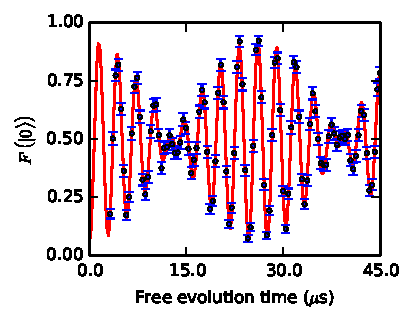
\includegraphics{Img/CarbonRamsey_C1.pdf}
    \caption{Nuclear Ramsey of Carbon 1} \label{fig:CR_C1}
    \end{subfigure}
    \begin{subfigure}[t]{0.49\textwidth}\centering
        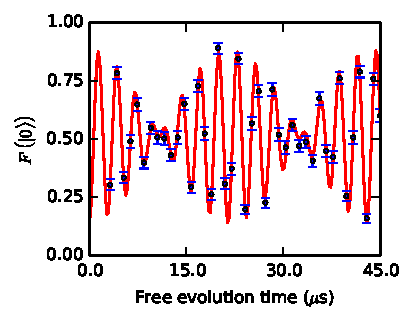
\includegraphics{Img/CarbonRamsey_C4.pdf}
        \caption{Nuclear Ramsey of Carbon 4}
        \label{fig:CR_C4}
    \end{subfigure}
    \caption{Nuclear Ramsey experiment wit}
\end{figure}


\subsubsection{Theory, what happens if }
\subsubsection{Experiment}



\subsection{Controlling a single carbon}



\subsubsection{Theory, initialization and readout}
\subsubsection{Single qubit tomography and T2*}

\section{Controlling multiple-carbons}
\subsection{The parity measurement}
\subsection{MBE}

\begin{figure}[htbp]
    \centering
\mbox{
\Qcircuit @C=1em @R=.7em {
\lstick{\ket{0}_e} & \gate{\mathrm{y}}  & \ctrl{1} &  \ctrl{2} & \gate{y}  &  \meter &\qw\\
\lstick{\ket{0}_{C1}} & \qw&  \gate{\pm \mathrm{x}}  &\qw  & \qw       &\qw&\qw& \\
\lstick{\ket{0}_{C2}}& \qw& \qw  & \gate{\pm \mathrm{x}}    & \qw      &\qw&\qw&}}
    \caption{XX-parity-measurement}
    \label{fig:gate_circuit_XX-parity-measurement}
\end{figure}

\begin{figure}[htbp]
    \centering
\mbox{
\Qcircuit @C=1em @R=.7em {
\lstick{\ket{0}_e} & \gate{\mathrm{y}}  & \ctrl{1} &  \ctrl{2} & \gate{\mathrm{y}}  & \ctrl{1} &  \ctrl{2} &  \meter &\qw\\
\lstick{\ket{0}_{C1}} & \qw&  \gate{\pm \mathrm{x}}  &\qw  &\qw  & \gate{\pm \mathrm{x}} & \qw   &\qw&\qw& \\
\lstick{\ket{0}_{C2}}& \qw& \qw  & \gate{\pm \mathrm{x}}    & \qw    &\qw& \gate{\pm \mathrm{x}}    & \qw &\qw&}}
    \caption{General parity RO}
    \label{fig:gate_circuit_general_Parity_RO}
\end{figure}






\section{Controlling weakly coupled carbons trough the electronic spin}
% Section containing theory (Gate circuits) on how to initialize and readout carbons

Explain how carbon control works in theory.
Explain how a conditional and unconditional gate can be performed.
Explain initialization on gate level, refer to appendix for calculations.
Explain Readout.

\subsection{Initialized Carbon Ramsey}


\section{Carbon Initialization \& Readout}
% TODO_MAR: Discuss naming of sec: Carbon Init&RO and Carbon Tomo
%  Section containing experimental results (Tomographies)
%  Should emphasize difficulty in seperating initialization and RO fidelity, what is not working? Is it working?
Show results that demonstrate carbon control.



